\documentclass[../main.tex]{subfiles}
\begin{document}

This chapter will serve as a guide for the thesis. Indeed, it will present the context to the reader by giving definitions and structure to the thesis. The goal is also to help the reader to build some tool in order to make their own opinion about the subject of this work. As the concepts introduce in the following pages are broad, only the main features will be presented. For further, more accurate details, see the appendixes at the end of the thesis.

First, there will be an introduction to international negotiations. What are the main elements, who is involved, what are the strategies. It is a broad concept, however, only the salient aspects will be covered, as this chapter serves as a base to understand better the issue of the whole work (for further explanations, see Appendix ? at page ?).

Next, the other main protagonist of this work will be presented: culture. Culture is a vast concept and has many facets and elements. But, also is this case, only the main characteristics will be taken into consideration (for further references, see Appendix ? at page ?).

Finally, the important part is to assess the structure of this thesis.
To make some order within the literature that exists on the subject and considering how vast it is, I decided to categorise the literature contemplated %se riesci a trovare un sinonimo è meglio
in this thesis following the streams of thought identified by Faure in his article "The Cultural Dimension of Negotiation: the Chinese Case" (1999).\\
\pagebreak

\subchapter{\textbf{The Concept of Negotiation}.}\\

Negotiating is something that we all in everyday life, it is just that we do not realise it. When making plans with friends about what to do for the night, when deciding with your significant other who is going to do the dishes, when settling a price of a car.
In international negotiations, things are not much different: they are just in a bigger scale. The following pages will give an insight and some definitions of what an international negotiation is.

In order to define what an international negotiation is, it is convenient to define the concept of "negotiation". To negotiate means, according to the Merriam-Webster dictionary, "to confer with another so as to arrive at the settlement of some matter"\footnote{\textit{Definition of Negotiate}. Merriam-Webster \url{https://www.merriam-webster.com/dictionary/negotiate}}. Hence, a negotiation is a process, a sequence of actions, in which the actors involved will try to reach a situation that is superior to the \textit{status quo} situation. An international negotiation is a negotiation that involves international actors, such as States, Non Governmental Organisations, Supranational Institutions (such as the European Union), etc.

\textbf{Actors.} The actors in a negotiation process can be either internal or external. The internal actors are the \textit{parties}, which are directly involved in the negotiation process and in its outcome: they have interests involved in the negotiation and they stand on a position during the process. Ideally, the position should be representing someone's interest, but a clarification needs to be made:
\begin{itemize}
\item Position: is what the actors say they want, that is what the actor choose to share with the other party. Positions are surface statements of where a person or organisation stands, and rarely provide insight into underlying motivations, values or incentives\autocite[]{watershed}.
\item Interest: is what really moves the process behind the fuss of position; the interest is a party's underline reason for the initiation of the negotiation in the first place and it reflects the values and the motivation of the parties. An interest can explain why a party choose a certain position but it does not mean that the position and the interest beneath it overlap.
\end{itemize}
The external actors, also known as \textit{third parties}, form a part of the negotiation structure but they are not directly involved in the negotiation: they don't have direct interest but they contribute to shape the outcome of the negotiation. There are three types of third parties: the \textit{Chair} of a negotiation, the \textit{Mediator}, and the \textit{External parties}. The Chair makes sure that actors follow he rules of procedures; the Mediator is a neutral and impartial actor whose goal is to smoothen the process by facilitating the communication between the parties; the External parties do not have an official role in the process, but somehow they have some interest in the outcome of the negotiation.

The negotiation process can be divided in four main stages:
\begin{enumerate}
\item \textbf{Status quo}: is the initial situation. It is usually a situation less favourable than the one after the negotiation is concluded. Nonetheless, sometimes actors prefer the status quo rather than an outcome that could be less favourable for them.
\item \textbf{Verbal exchange}: is the reason why and in what ways the parties talk to each other. In this stage, information are exchanged between the parties.
\item \textbf{Strategy}: is the intellectual line of action that a party will adopt in order to maximise its payoff of the negotiation. According to Pruitt, there are four types of negotiations strategy, as he explains in his article "Strategic Choice in Negotiation"\autocite[167]{pruitt}.
\item \textbf{Tactic}: all the actions used to implement the strategy adopted. The entirety of all the tactics used by the parties compose the strategy.
\end{enumerate}

One other contribution on the division of the negotiation process is provided by Zartnam and Berman in their book \textit{The Practical Negotiator}. They describe the negotiation process as a process in which divergent values are combined into an agreed decision, and it is based on the idea that there are appropriate stages, sequences, behaviours, and tactics that can be identified and used to improve the conduct of negotiations and better the chances of success \autocite[2]{zartman1982practical}. They divide a negotiation process in three stages: diagnostic phase, formula phase, and detailed phase. These stages are not isolated, indeed they sometimes overlap.

The diagnostic phase feature the definition of the situation in which the parties explore the possibilities of negotiating. According to Zartnam and Berman, a negotiation will be due when the a situation that is already not positive for the parties will become worse in the future if no action is taken.

In the formula phase, the parties have agreed to proceed with the negotiation reaching a point that is called \textit{Turning Point of Seriousness} \autocite[3]{zartman1982practical}: that is when each parties realises that the other is serious about jointly work to find a common solution. Indeed, the parties will try to search a general principle that will serve as a guideline for the entirety of the negotiation.

During the detail phase the negotiation are going to focus on the assessment of the details for the implementation of the formula they agreed. According to Zartman and Berman, one of the most important thing in a negotiation should be the high level creativity of the parties that corresponds to  the way negotiators handle concession-making situations.

The strategies implemented can be many. In general, parties will adopt three kind of strategies. Sometimes they will combine strategies if the situation requires so. The main strategies are:
\begin{itemize}
\item \textbf{Yelding}: a party will diminish its own demands and will concede. Therefore, an agreement will be found, but at the expenses of the party that implements this strategy. This strategy is implemented mostly when the the issue is not relevantly important and there is the presence of high time pressure.
\item \textbf{Problem Solving}: it is a strategy based on collaboration. By adopting this approach, parties will cooperate in order to identify solutions that will satisfy everyone's goals. In order to do so, various formulas are available, such as: expanding the pie (parties will find a way to increase resources that have been in short supplies), cost cutting (one party gets what it wants by cutting the other's cost of conceding), compensation (a party rewards the other for conceding), logrolling (each party concedes on issues that have low priority to themselves), and bridging (a new option is developed that satisfies both parties' aims) \autocite[168]{pruitt}.
\item \textbf{Contending}: a party will pursue its goal without making concessions by tying to make the other party to concede. By adopting this type of strategy, the actors show themselves as competitive: this results in a lower chance to find an agreement than it would have been by adopting other strategies.
\item \textbf{Inaction}: it means that the parties will do as little as possible. This type of strategy often wastes time and sometimes it even suspends temporarily the negotiation \mancite\autocite[172]{pruitt}.
\end{itemize}

To summarise, the main protagonists of a negotiation are the parties directly involved. In order to find an outcome, the parties will start to exchange proposals until an agreement will be found. There are many elements to consider and there are many strategies that can be implemented.

Of course, there are many factors that influence the negotiator during the implementation of a strategy. Those factors refer to the structural context, to the personality of the actors, or of their culture. Indeed, this is the main focus of this thesis. However, before getting into it, it is necessary to analyse the concept of culture.
\pagebreak

\subchapter{\textbf{The Concept of Culture}.}\\

Culture is arguably one of the most difficult concepts to delineate. What is culture? How can it be determined? What are its borders? These questions are very complicated to answer. But, for the purpose of this thesis' topic, I will try to define and mark the borders of the concept. In order to do so, I will appeal to the article of Helen Spencer-Oatey: "What is Culture? A compilation of Quotations"(2012), in which she orderly makes some considerations about culture and collects quotations from the most famous scholars. Only the points relevant for this thesis will be considered. For the entire analysis, see Appendix ? page ?.

Culture can be perceived from different things: a painting, a habit, a behaviour. Sometimes we do not even realise that an action embedded in our routine comes from our cultural background. 
This differentiation of manifestation of culture comes from the fact that culture is made of layers \autocite[3]{schein}.
Those layers are: observable facts, values, and basic underlying assumption (Figure \ref{fig:schein}).
\begin{figure}[h]
    %\centering\includegraphics[width=0.8\textwidth]{images/cafoscari.png}
    \centering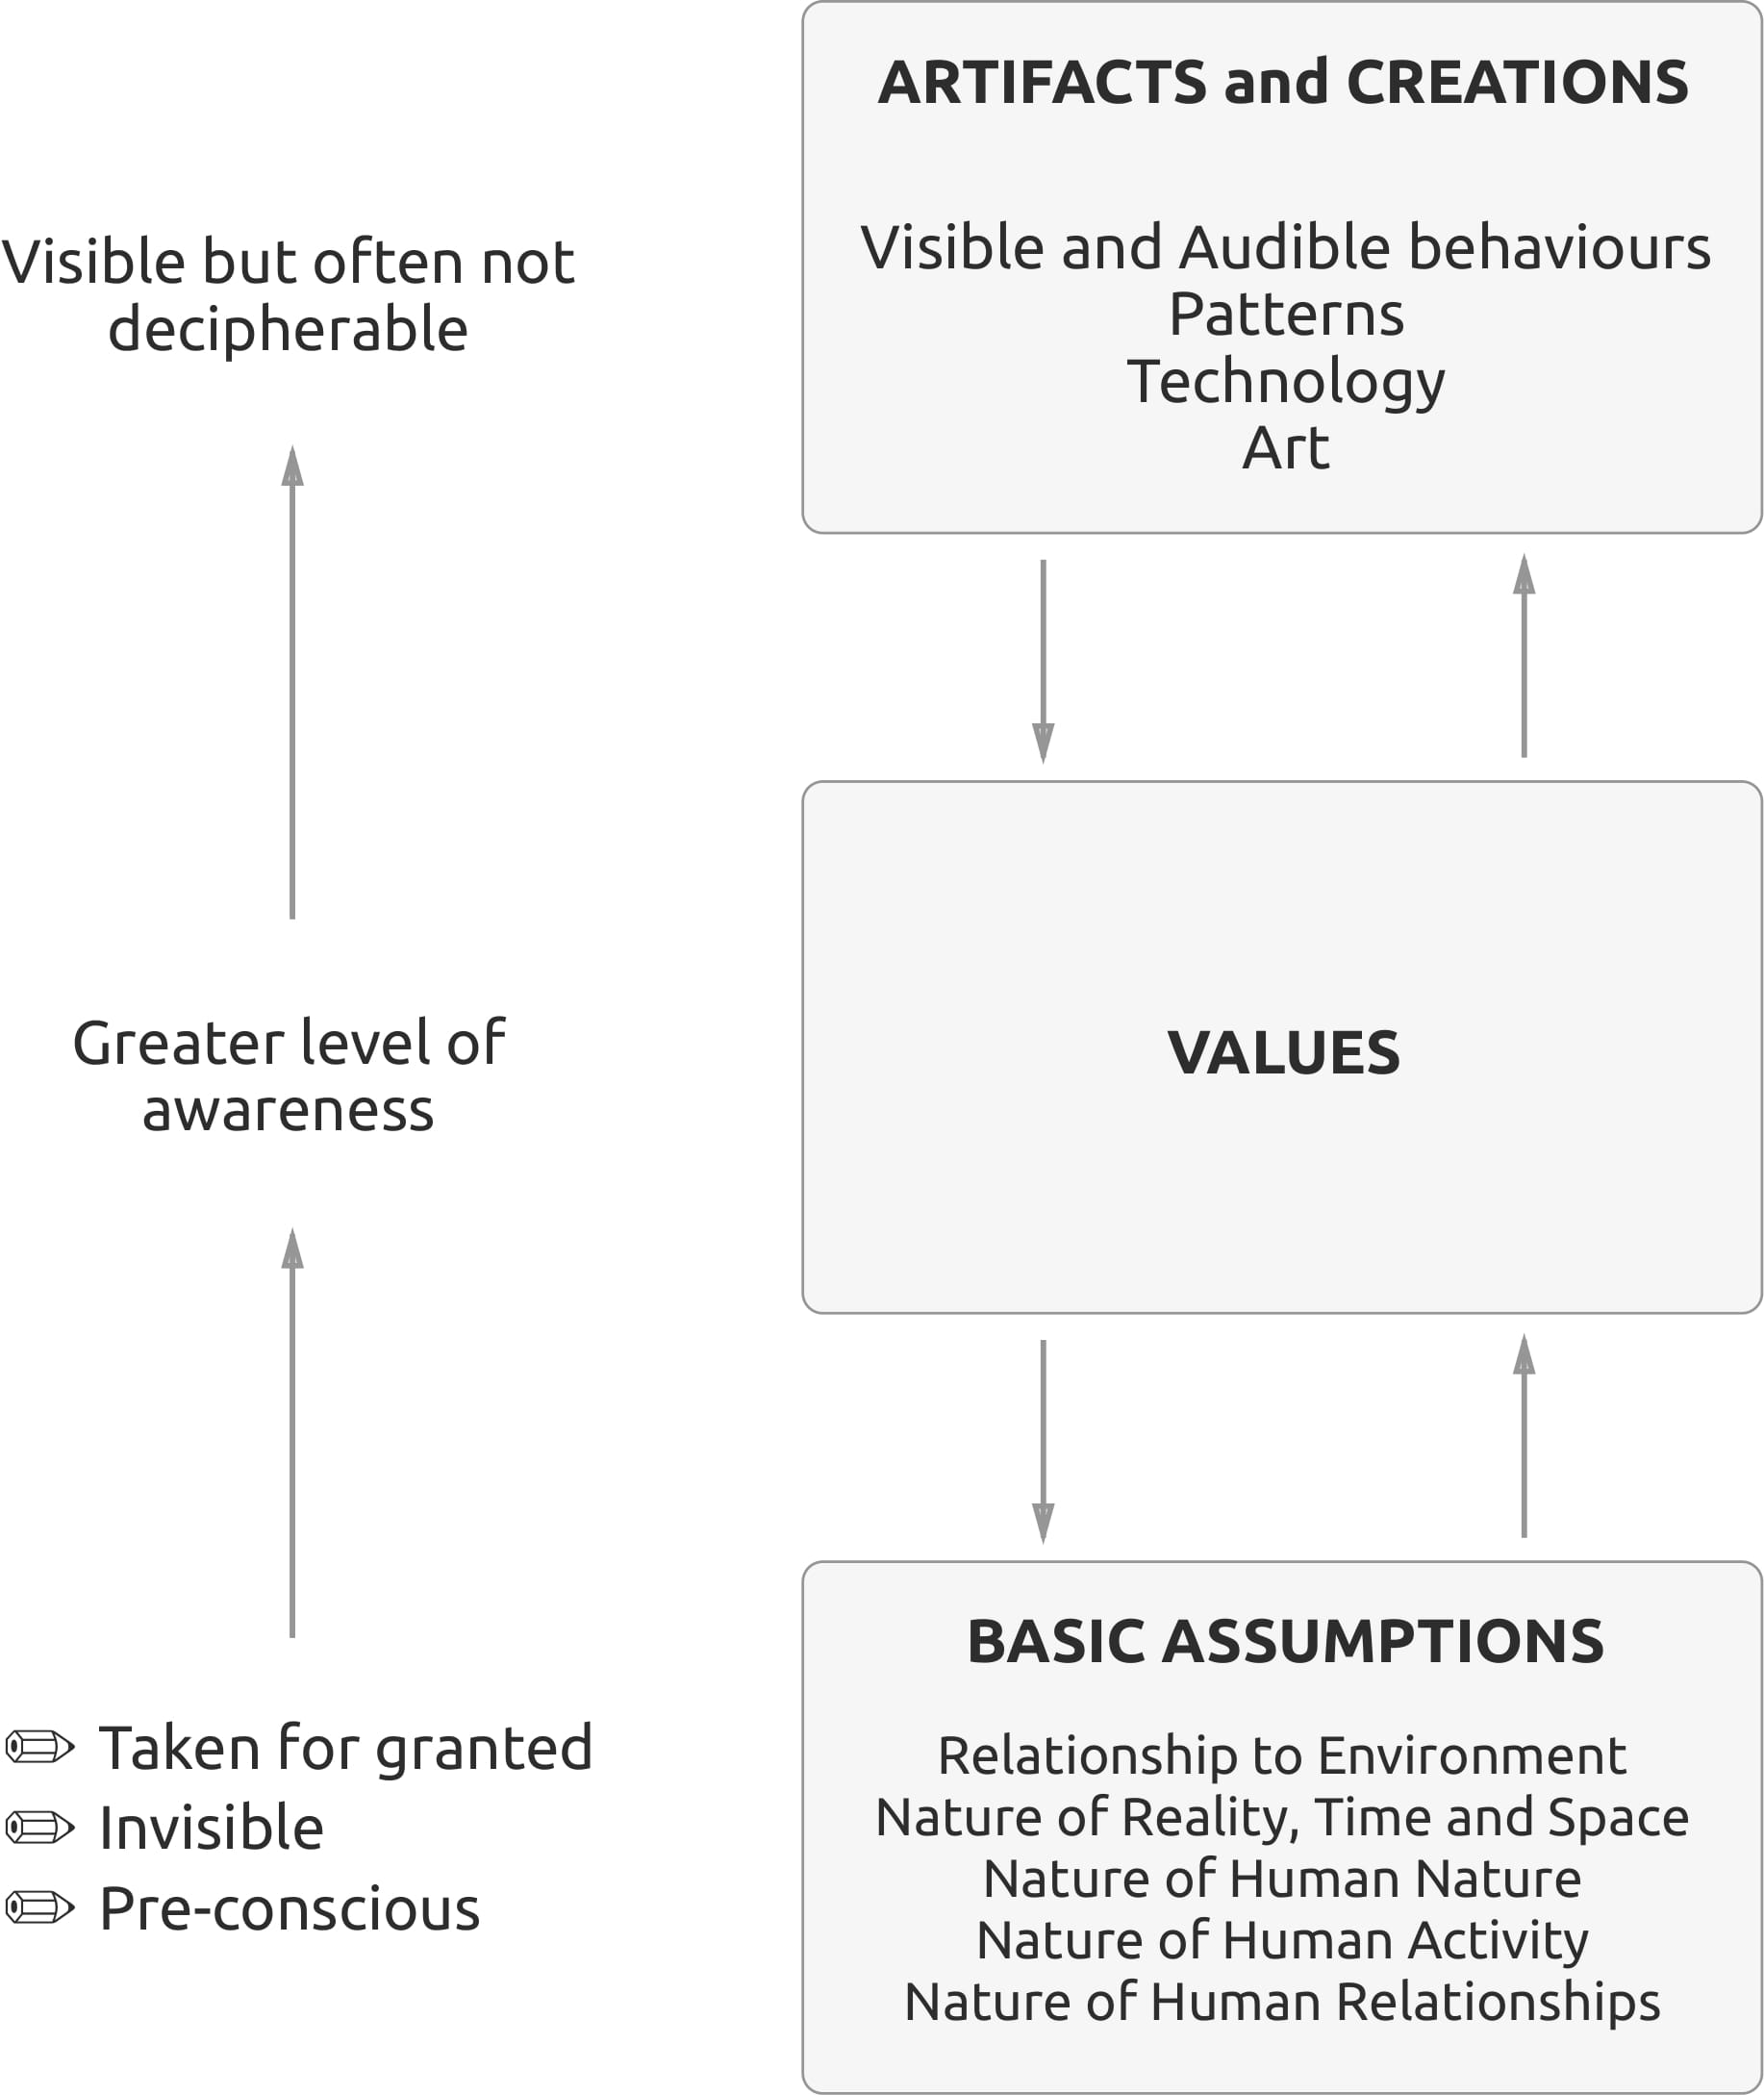
\includegraphics[width=0.45\textwidth]{images/values}
    \caption{Schein's model: levels of culture \autocite[4]{schein}.} %scrivi ammodino la didascalia poi eh
    \label{fig:schein}
\end{figure}
The first one relates to the surface, to what is visible: here data is very easy to acquire but difficult to interpret. To put it in other words, by looking at the observable facts, we can understand "what" are the behavioural norms followed and "how" the group builds the surroundings, but we cannot understand "why" a group adopts a specific behaviour. To answer the question of "why" a group of people adopts certain behaviours, we need to take into consideration the values, that compose the aforementioned second layer. However, values represent only the espoused values of a culture: this means that they unveil only what people \textit{say} it is the reason for their actions. Therefore, the real motivations remain obscure or unconscious. To solve this issue, it is necessary to appeal to the basic underlying assumptions. Those assumptions are themselves a sort of learned responses that were originally espoused values \autocite[3]{schein}. However, as values lead to a certain behaviour and behaviours are a manifestation of a culture, values turns into an underlying assumption about how things really are. Once the assumption is established and, therefore, taken for granted, it abandons consciousness. Assumptions that are taken for granted are powerful because are less keen to be a subject of debate than espoused values. When dealing with an underlying assumption, it will be hard to find someone willing to discuss the reason behind it. For example, the belief that a business should be profitable is something that we assume is the right way of doing business but actually we cannot explain exactly when we learned that notion, we just know it. The result of Schein suggestion is that, in order to visualise the effects of culture on international negotiations, it is necessary to search for the behaviours, then the values, and, eventually, those will lead to the underlying assumptions \mancite\autocite[4]{schein}.

It is important to acknowledge the fact that culture can manifest itself through subconscious patterns because, in international negotiations, parties will make assumption on what is thought to be a universal principle (for example, the concept of time), whereas it is a subconscious reflex of what it once was an acknowledged value.

Speaking of universal principle, it is important to remark that culture can be discerned between universal human nature and unique individual personality \autocite[6]{helen}.

As Hofstede points out, culture is learned not inherited. This is a very important remark because it implies that culture does derive from the social environment and it is not something that comes from the genes. Moreover, culture should be differentiated in human nature, on one side, and in an individual's personality, on the other. Nonetheless, the border between those two concepts is very blurry and it is still object of discussion. Hofstede identifies three levels of uniqueness in the human mental programming (Figure \ref{hofstede}):
\begin{figure}[h]
    %\centering\includegraphics[width=0.8\textwidth]{images/cafoscari.png}
    \centering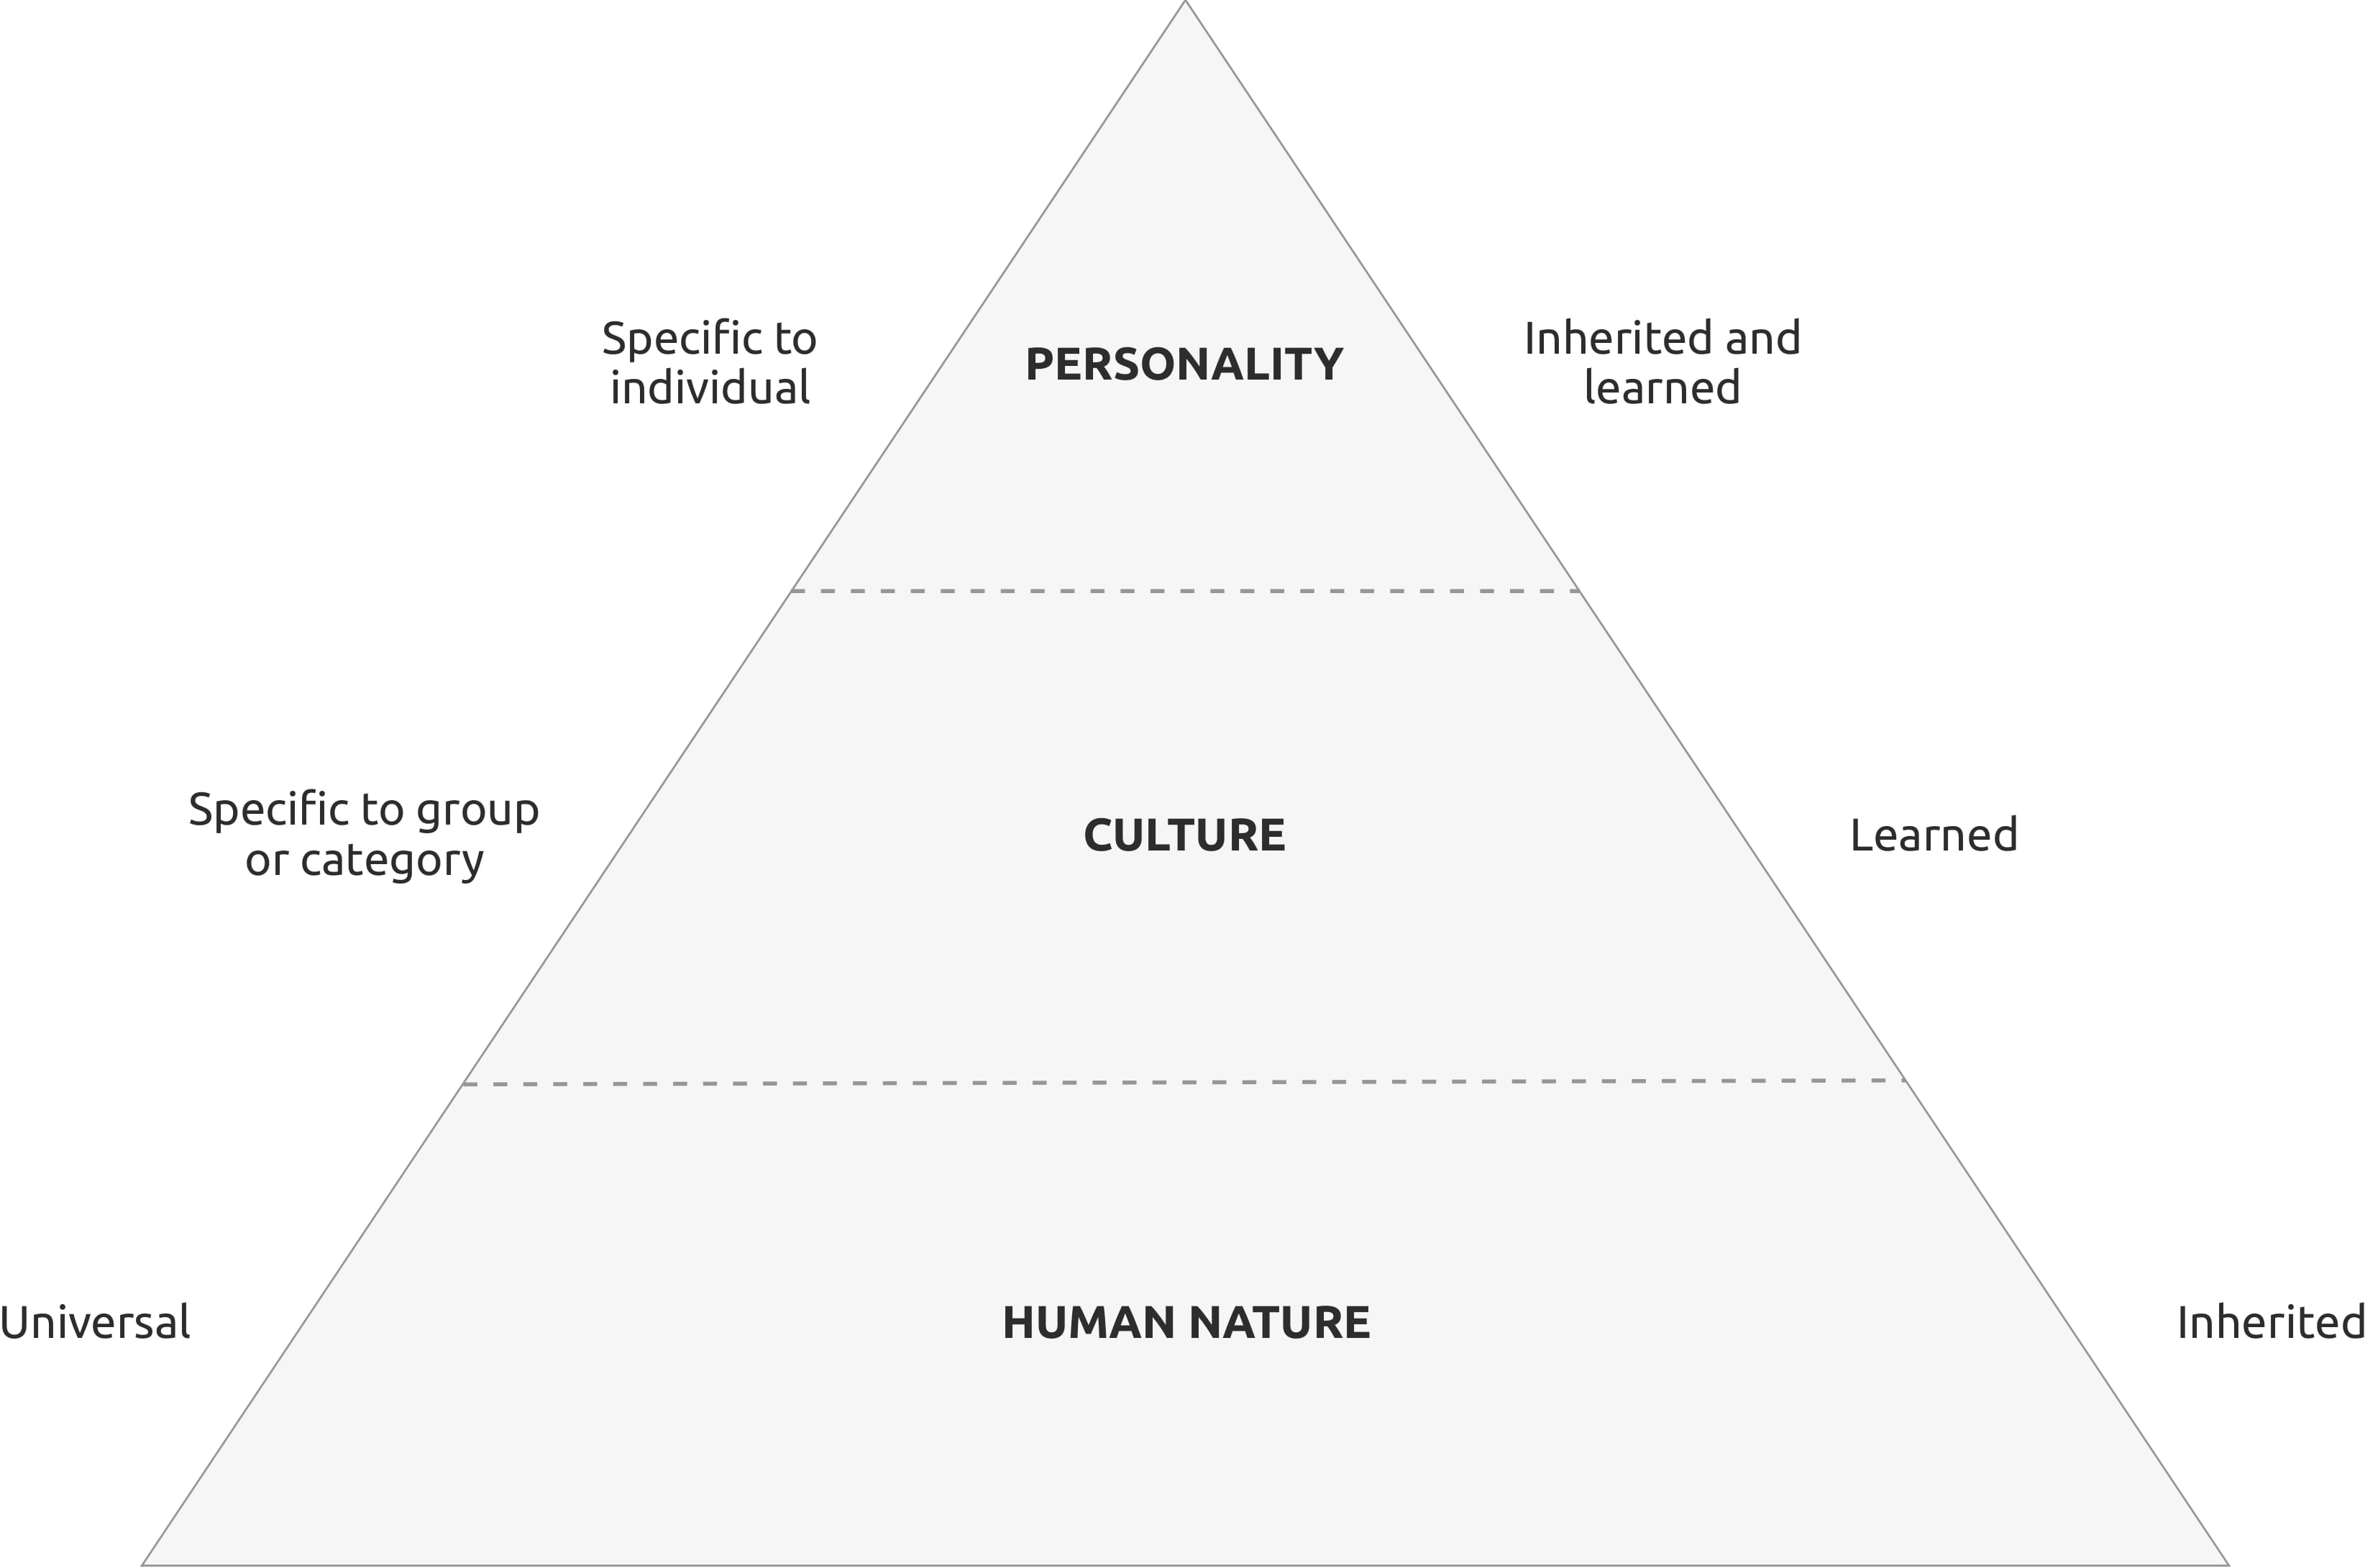
\includegraphics[width=0.6\textwidth]{images/levels-1}
    \caption{Hofstede's model: levels of mental programming \autocite[6]{hofstede}.}
    \label{hofstede}
\end{figure}

\textit{Human nature} is maybe the only thing that all human beings have in common: this level is inherited from one's genes and it relates to one's physical and basic psychological functioning. For example, the human ability to perceive feelings or the basic needs, such as the need to associate with others. However, the way in which the feelings are expressed and how an individual associates with others is affected by culture. Most of the aspects related to this level concern also the animal kingdom when there is a reference to primal instincts. On the other hand, the \textit{personality} of an individual is their personal set of mental programming that do not share with anyone else. It is a combination of human nature deriving from one's genes and of something learned through both culture and personal experiences. Historically, cultural assets have been linked with heredity because scholars could not find a better explanation for the outstanding differences in cultural patterns among different civilisations. But, the role of hereditary has been amplified in the "theories" about race which somehow have been used to justify, over the course of history, cultural superiority and inferiority\footnote{It is sufficient to think about how the feeling of being a "superior" race led to despicable events, such as the Holocaust, the Apartheid, the racial laws that existed in the US against African-American people.}.

Therefore, what it is important to assess in a negotiation is the culture of a negotiator which stands between their human nature and their personality. Personality is the deceiving feature because it can be dealt with as culture when, in reality , it is not.

One more thing that needs to be pointed out is that culture is associated with social groups \autocite[7]{helen}. Hofstede identifies many levels of culture:
\begin{itemize}
\item National level according to one's country (or \textit{countries} for people who migrated);
\item Regional/ ethnic/ religious/ linguistic affiliation (as most nation are composed of culturally different groups);
\item Gender level;
\item Generation level, which separates different kin generations;
\item Role category (e.g. parent, son/daughter, teacher, student);
\item Social class level, associated with educational opportunities and with a person's occupational profession;
\item Organisational or corporate level, according to the way employees have been socialised within their working environment. \autocite[18]{hofstede}
\end{itemize}
Hofstede also notes that, especially in modern society, many layers are in conflict with each other. For example, religious values may conflict with generation values. As a result of these conflicts in mental programming, anticipating the behaviour of people in a new situation gets challenging.

Other authors give their contribution, such a s Salacuse in his article "Ten ways that Culture Affects Negotiating Style: Some Survey Results" (1998). He defines culture as "the socially transmitted behaviour patterns, norms, beliefs and values of a given community." \autocite[222]{salacuse}. Indeed, for the purpose of his article, he makes a distinction between national culture and professional or occupational culture. The professional background forms a subculture of some sort, therefore it is necessary to take it into consideration.

In his article, he takes on a survey and analyses both national and professional culture of the participants (the nature of the article will be discussed in details in the next chapter).

For the purpose of this thesis, however, these distinctions concerning the different layers of mental programming (in Hofstede's words) will not be contemplated as, in an international diplomatic negotiation, the negotiators are thought to belong (more or less) to the same professional, generational, social class background. Therefore, the cultures that are taken into consideration in this work are the one belonging to a country\footnote{For the scope of this work, a country is considered an homogeneous entity enclosed within its current political border.}. From now on, the focus will be on national culture (mentioned as just culture).

Since it is possible to acknowledge other cultures, it is also possible to learn them: culture is learned through the people you interact with. Ferraro informs us that this concept causes many implications. First, saying that culture is learned implies that an individual can also learn about other cultures: this will lead to a greater tolerance and understanding, therefore leading to a better communication with others. Second, since we learn culture, it is possible for an individual not only to function in their own culture, but also in other cultures. Third, foreign work forces lacking certain job related skills are capable to learn those skills in the future \autocite[19]{ferraro}.

And if people can learn about other cultures, they can also borrow traits from them. Therefore, Culture is subject to gradual change \autocite[12]{helen}.

We cannot think that culture is a static concept.
It is essentially fluid and constantly in motion. This makes it so that it is difficult to define any culture in only one way in the first place. Ferraro \autocite*[25-29]{ferraro} helps us once again to understand better this concept. First of all, mechanisms of change within a culture are called \textit{discovery} and \textit{invention}. Nonetheless, most innovations introduced into a culture are the result of borrowing from other cultures. This process is called cultural \textit{diffusion}, meaning the permeating of cultural elements from one culture to another.

Why this happens? It is merely an explanation in term of economy of effort: indeed, it takes less effort to borrow someone else's invention rather than making it from scratch. Cultural diffusion varies from situation to situation but there are some stable elements worth mentioning.

First, cultural diffusion is a selective process. This means that cultures do not borrow every item from other cultures indistinctly. If so, the difference among cultures would have eventually disappeared. Rather, cultures borrow from other cultures the items useful for them and that result compatible with their own characteristics. Therefore, an item will be taken into consideration if it is seen superior to the existing one, it is consistent with the cultural pattern, it is easily understandable, it can be tested on an experimental basis, and it provides clear benefit that can be seen from a large group of persons.

Second, culture diffusion is a reciprocal process. It means that when two cultures get in touch with each other, \textit{both} cultures will borrow something from the other.

Third, it is very rare that the items cultures borrow from other cultures are embedded within the culture in the original form. Every item goes through a process of reinterpretation in order for it to be more effectively and more efficiently integrated into the total configuration of the borrowing culture. As an example, let us take into consideration the food par excellence: pizza. Pizza is notoriously a wide-world recognized Italian dish, however it has been adopted by cultures all over the world. Originally, pizza is made with mozzarella, tomato sauce, oregano, on a crust made of water, flour, oil, and yeast. However, in some cultures, oregano is considered too spicy, therefore the dish has been reinvented to meet the taste of other cultures. In some countries it is topped with processed cheese instead of mozzarella and the oregano has been left out. Or in some other occasions, the toppings chosen are very far from the original ones. Such as the choice of putting pineapple on pizza. Even if an Italian person would not recognize as legitimate a pizza with pineapple on it, they would still call it pizza.

\begin{figure}[h]
\centering
\begin{subfigure}{.5\textwidth}
  \centering
  
\includegraphics[width=.53\linewidth]{images/margherita.png}
  \caption{Pizza.}
  \label{fig:sub1}
\end{subfigure}%
\begin{subfigure}{.5\textwidth}
  \centering
  
\includegraphics[width=.5\linewidth]{images/hawaii.png}
  \caption{"Pizza".}
  \label{fig:sub2}
\end{subfigure}
\end{figure}

Fourth, some cultural traits are more easily diffused than others. Logically, technological innovations are more likely to be borrowed than social patterns. For instance, it is easier to convince a man that a car will carry you faster than by walking on foot; however, it will be more difficult to convince a Hindu person to switch to socialism.\\


Culture is a vast concept that is not possible to describe and analyse thoroughly in just few pages. Culture hides and, at the same time, manifest itself through a gesture, a word, a behaviour. Culture is intricate, yet intuitive. It has many aspects to be acknowledged in order to have a at least a partial conception of it. However, some remarks are important to make, in order to keep going with this work. Culture has many layers, as it can relate to gender, age, professional environment, social class. But, as stated before in this chapter, as the focus in on negotiations, negotiators are thought to belong to the same (or almost the same) group concerning age, social class, professional environment. Therefore, what matters, what stands out is the difference in national cultures. In recent times, though, with globalisation, it is easier to see that cultures are diffusing among them, meaning that they borrow traits and inventions from one another and this leads to some sort of homogenisation concerning some aspects.
A good negotiator might get to know the culture of their counterpart before meeting them, since culture can be learned. Indeed, when confronting a party from another culture, a negotiator can learn about the other party's culture and be prepared for differences and divergences. Hence, it is possible to restrain potential disagreements. What is important to remember is that the intentions of the negotiators are all the same: to reach an agreement in the smoothest way. The issue come when it is time to manifest the actions in order to reach the desired effect. That is when culture does its part and leads to different approaches and behaviours.

For the purpose of this thesis, this analysis of culture is sufficient to understand what relies under this notion. It is, indeed, a very broad, rich, varied conception which still today causes debates over its nature, its definition, its characteristics. But, as much as it is an interesting and fascinating debate, the clarifications made in this chapter are enough for the usefulness of this thesis.
\pagebreak

\subchapter{\textbf{Culture and Negotiation across Research.}}

In the previous pages, there was an analysis of the concept of negotiation and the concept of culture. The hope is that the analysis will provide the reader some tools and definitions to better comprehend this chapter. Indeed, in these next pages, there will be an analysis of the literature concerning the influence of culture on negotiation. The main subject of this work is international \textit{diplomatic} negotiations but, since culture affects negotiations on common features regardless of whether it is a diplomatic one or not, also scientific works on other types of negotiations will be included as a theoretical base for this thesis.%riguarda discorso

Considering the remarkably vast literature that exists on the subject, I decided to categorise the literature contemplated %se riesci a trovare un sinonimo è meglio
in this thesis following the four streams of thought identified by Faure, in his article "The Cultural Dimension of Negotiation: the Chinese Case" (1999). In the article, he addresses the work of Hofstede and also tries to categorise the cultural studies. Particularly, Faure identifies four main streams of approaches on the research on international negotiation that focuses on cultural aspects.
\begin{enumerate}
\item \textbf{Structural-processual approach}: it relies on the model of Sawyer and Guetzkow. Since it was not possible to trace the original model, it is sufficient to say that it is based on a set of variables intervening in a negotiation. This approach tells us that culture is either perceived as integrated within the factors that compose the context of the negotiation, or it acts through each analytical category (contextual or situational, processual or behavioural, strategic or related to the outcome).
Under this approach, Faure cites a book written by Rosalie Tung called "U.S.-China Trade Negotiations" and the article "Analysis of Complex Negotiations in International Business: The RBC Perspective" written by Stephen Weiss.
\item \textbf{Behavioural approach}: under this approach, two different methodological traditions have been established. The first one aims at assessing the impact of culture on a number of behavioural variables. The second one is based on surveys and focuses on describing the influence of culture on the behaviour of the negotiators.

The authors cited under the first stream are: Carnevale and his article "Property, Culture, and Negotiation" that approaches the issue under the individualist/collectivist cultural opposition. Kirkbride, Tang, and Westwood with their article “Chinese Conflict Preferences and Negotiating Behaviour: Cultural and Psychological Influences”; then, Trompenaars' book "Riding the Waves of Culture: Understanding Cultural Diversity in Business". The last author quoted under the first stream is Hall with his book "Beyond Cultures".
Under the second stream, the article mentioned is "The Influence of National Culture on Negotiating Style: A New Zealand-UK Perspective", written by Dr Anna Zueva, Dr Helen Rogers, Jemma Corbett, and Virginia Cathro.

\item \textbf{Cognitive-strategic approach}: it intends to study the connection between a negotiator's action and their mindset in order to disclose the logic implemented during the negotiation.
There are three articles mentioned: “Negotiating with Foreign Business Persons” written by Stephen Weiss and William Stripp; the second article mentioned is “Negotiation: the Chinese Concept” written by Faure himself; the third article is "Ten Ways that Culture Affects Negotiating Style: Some Survey Results" by Salacuse (already mentioned in Chapter \ref{chap:3}).
\item \textbf{Stages approach}: within this framework, negotiations are divided in stages with different requirements. The satisfaction of the requirements in each stage allows the the adjustment on the different sequences and the reaching of the agreement.
Two main articles will be analysed: "The Global Negotiator Making, Managing, and Mending Deals Around the World in the Twenty-First Century" written by Salacuse, and "The Negotiation Dance: Time, Culture, and Behavioral Sequences in Negotiation" written by Adair and Brett.
\end{enumerate} %riguarda tutto perché va citato ammodo eh!!!

Faure already includes some authors in his article, dividing them in the categories he has identified. However, for the authors that are not mentioned in the article and that I have arbitrarily considered and included in this thesis, there will be an explanation for the reason why they are inserted within a specific approach.

\end{document}